% AUTHOR: Ruslan Kiianchuk <ruslan.kiianchuk@gmail.com>
%

\chapter{State of art analysis and synthesis of symmetric cryptographic transformations}
\label{sec:symmetry_review}

Evaluation and design rationale are essential parts of developing and
deploying  the considered cryptographic security system. The primary goal of
cryptography is to design mathematical methods for providing security against
adversary's malicious actions under any predetermined conditions.

However, as practice shows, it's unfeasible to take into account all possible
attacks that may be invented in the future due to technological and scientific
innovations during the development stage. Therefore, the most widespread
method for analysing computationally strong cryptographic primitives is
complexity evaluation of every known applicable attack.

\section{Classification of attacks on symmetric ciphers}

Attacks on symmetric ciphers are defined by the abilities and data
that an adversary can operate with. Most of them refer actions that may be
done to cipher entities such as plaintexts and ciphertexts, however a separate
class of attacks that exploits cipher implementation rather than the
algorithm itself exists.

A ciphertext-only attack leaves the adversary with a set of ciphertexts that
she
\footnote{Following the tradition started by Shafi Goldwasser in her Lecture
Notes on Cryptography, ``she'' is used throughout the text as referring to a
subject of unknown gender.}
can use to recover the corresponding plaintext or encryption key. Such
conditions are the most complex for cryptanalyst. In a known plaintext attack
the adversary has a fixed set of plaintext and ciphertext
pairs~\cite{menezes:applied_cryptography}.

In chosen plaintext and chosen ciphertext attacks the adversary gets an
ability to encrypt plaintexts or decrypt ciphertexts of her choice
respectively. So the cipher needs to have such plaintext and ciphertext
spaces that would make it infeasible for the attacker to get full dictionary of
all possible plaintexts and corresponding
ciphertexts~\cite{menezes:applied_cryptography}.

Related key attacks exploits possible relations between encryption keys to
break the cryptographic system~\cite{StampLow:AppliedCryptanalysis}.

Side channel attacks are somewhat outside of mathematical attacks scope. They
use some cipher implementation peculiarities to gain information about the
encryption key observing the cryptographic system during operation. So far no
mathematical countermeasures exist that would guarantee the security of the
transformation against these types of attacks ~\cite{Quisquater:sidechannel}.

A cipher is considered to be insecure if any type of attack exists that allows
to get some information about the key with a complexity lower than a brute
force.

\section{Block ciphers}

A block cipher is a function which maps $n$-bit plaintext blocks to $n$-bit
ciphertext blocks, parameterized by a $k$-bit key
$K$~\cite{menezes:applied_cryptography}. Here $n$ is called the blocklength.
The encryption key $K$ has to be random. In order to always provide unique and
correct decryption the mapping function defined by a chosen key must be
bijective.

A straightforward usage of a block cipher to encrypt separate blocks of data may have
disadvantage in many applications. Consequently, several block cipher modes of
operations have been developed to satisfy various security purposes.

\subsection{Algebraic representation}
\label{sec:block-algebraic}

A symmetric block cipher may be represented as an algebraic
system~\cite{babash:cryptography}
\begin{equation}
\label{eqn:block-algebraic}
\Sigma_{A} = \left< X, K, Y, E, D \right> \enspace,
\end{equation}

    where $X$ is a plaintext space defined over finite alphabet $Q_X$, \\
$K$ --- a key set (usually defined by fixed length strings over $Q_X$), \\
$Y$ --- ciphertext space defined over finite alphabet $Q_Y$, \\
$E: X \times K \rightarrow Y$ --- a set of enciphering rules based on
parametrized maps $e_k(x) = y$ for which $k \in K$, $x \in X$, $y \in Y$. \\
Mappings $e_k(\cdot)$ and $d_k(\cdot)$ for any $k \in K$  are bijective and
ensure satisfaction of both conditions $d_k(e_k(x)) = x$ and $e_k(d_k(y)) = y$.
Plaintext and ciphertext spaces of all widespread modern symmetric ciphers
coincide ($Q_X = Q_Y$), so such ciphers are therefore endomorphic, that is
\mbox{$X = Y$}.
For cryptographically secure ciphers the sets of encrypting and decrypting
rules must have random mapping properties, and $e_k(\cdot)$, $d_k(\cdot)$ must
be random permutations.


\subsection{Modes of operation}

Simple encryption of data chunks block-by-block is called an electronics
codebook mode (ECB). As seen from figure~\ref{fig:mode-ecb} each plaintext is
encrypted independently. Error propagation is limited within one block, but
this mode is insecure for enciphering large correlated
data~\cite{menezes:applied_cryptography}.
\begin{figure}[htbp]
	\centering
	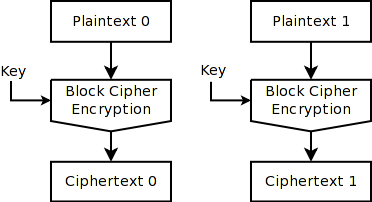
\includegraphics[scale=0.6]{images/modes_ecb}
	\caption{ECB mode of operation}
	\label{fig:mode-ecb}
\end{figure}

Cipher block chaining mode (CBC) is represented on figure~\ref{fig:mode-cbc}.
In CBC mode two identical plaintext do not encrypt to the same ciphertext as
the encryption depend on the initialization vector (IV) and two previous blocks
instead. This causes error propagation in ciphertext expand to two blocks, but
modifications to plaintext influence all subsequent blocks and make correct
decryption impossible. Such encryption mode is also more secure for enciphering
correlated data~\cite{menezes:applied_cryptography}.

Cipher feedback mode (CFB) shown on figure~\ref{fig:mode-cfb} turns a block
cipher into self-synchronizing
(see section \ref{sec:stream_ciphers_classification}) stream cipher.
\begin{figure}[htbp]
	\centering
	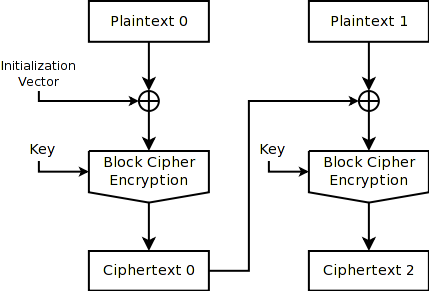
\includegraphics[scale=0.6]{images/modes_cbc}
	\caption{CBC mode of operation}
	\label{fig:mode-cbc}
\end{figure}
\begin{figure}[htbp]
	\centering
	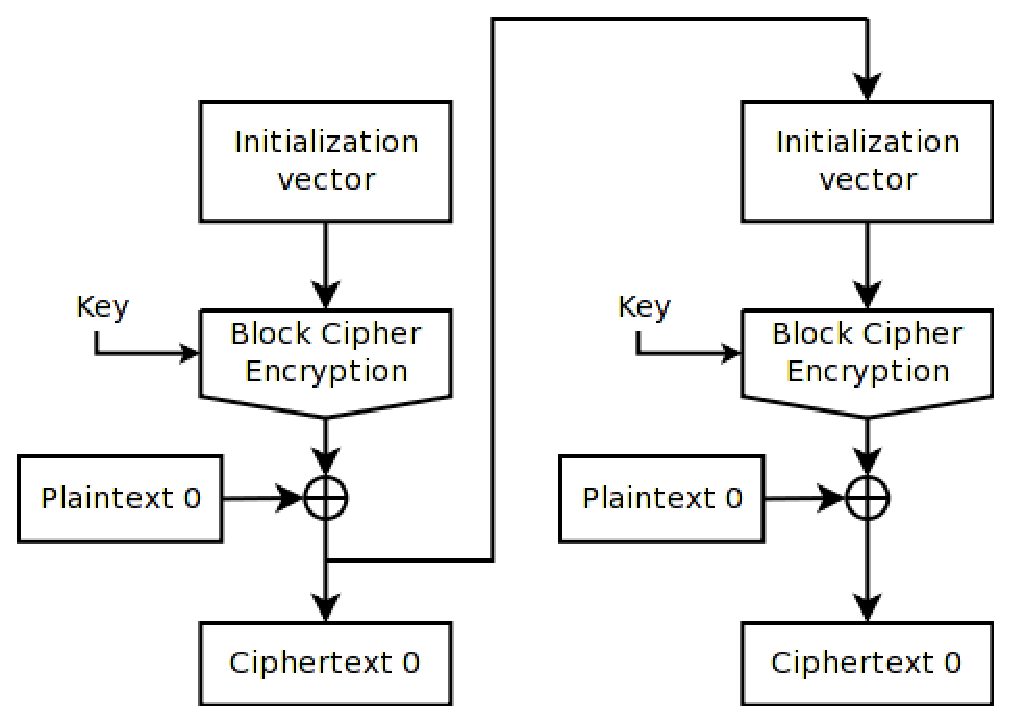
\includegraphics[scale=0.6]{images/modes_cfb}
	\caption{CFB mode of operation}
	\label{fig:mode-cfb}
\end{figure}

Output feedback mode (OFB) is similar to CFB (figure~\ref{fig:mode-ofb}) and
differs only by a feedback connection.
\begin{figure}[htbp]
	\centering
	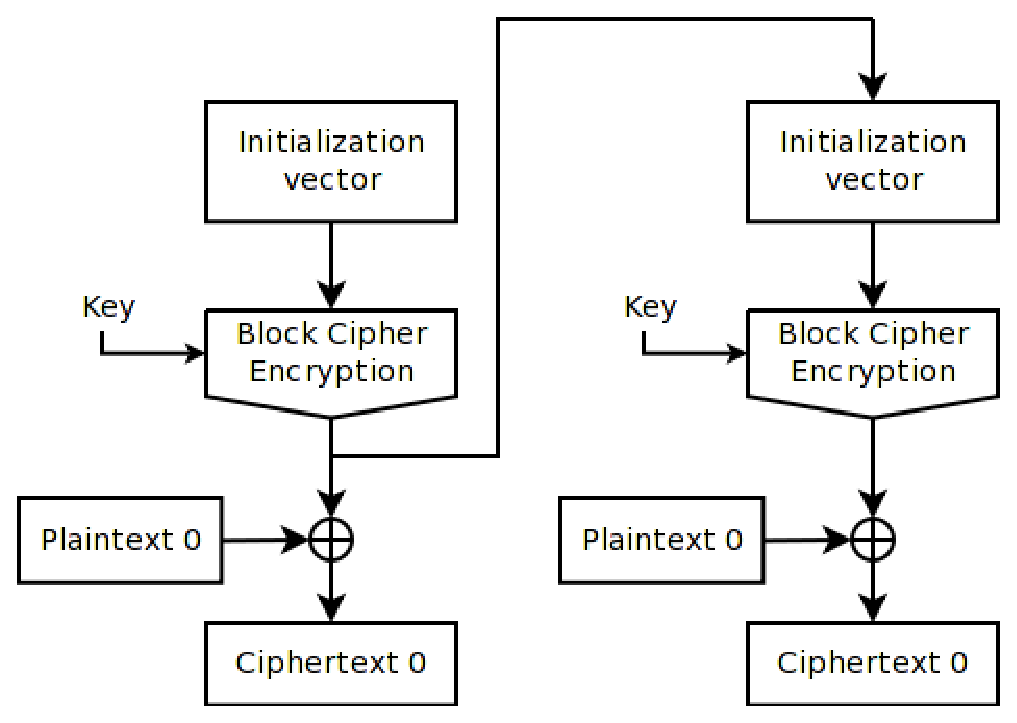
\includegraphics[scale=0.6]{images/modes_ofb}
	\caption{OFB mode of operation}
	\label{fig:mode-ofb}
\end{figure}
The main advantages of this mode is
absence of error propagation (since keystream generation doesn't depend on the
plaintext) and parallel processing capability.

\section{Stream ciphers}

The distinct difference between stream ciphers and block ciphers was for the
first time defined by Rainer Rueppel~\cite{robshaw:rsa:streamciphers}:

``Block ciphers operate with a fixed transformation on large blocks of
plaintext data; stream ciphers operate with a time-varying transformation on
individual plaintext digits''.

Stream ciphers gained great progress since Shannon's analysis of the
Vernam cipher where he proved it to be theoretically
unbreakable~\cite{shannon:secrecy}. However such cryptosystems were complex and
unprofitable to implement because of the need of secret channel to exchange key
material which was the size of the message itself.

Trying to overcome disadvantages of the Vernam cryptosystem, stream ciphers
inherit its idea, but use short key instead to generate a pseudo-random sequence
of needed length. That is, plaintext is encrypted into ciphertext with
pseudo-random sequence,  called the keystream, which is produced by a finite
state automaton whose initial state is determined by a secret key. Therefore
stream ciphers require high structural secrecy in order to be cryptographically
strong.

Stream ciphers are fast and well suited for hardware though some
cryptoalgorithms designed for efficient software implementation exist. They are
generally used in cases of continuous or unknown amount of data to be encrypted
and strict buffering constraints.

\subsection{Classification}
\label{sec:stream_ciphers_classification}

Depending on the choice of how the next state of cryptosystem is generated from
the current state, two types of stream ciphers are distinguished: synchronous
and self-synchronizing (or asynchronous)~\cite{menezes:applied_cryptography}.

In synchronous stream ciphers the next state of the automaton is independent of
plaintext and ciphertext. Such ciphers have no error-propagation and
consequently don't detect errors during decryption. This fact allows an attacker
to inconspicuously alter ciphertext which will be successfully decrypted to a
different plaintext. Another significance consists in the fact that encrypting
and decrypting devices must constantly stay synchronized. Otherwise the
decryption will fail.

Asynchronous stream ciphers are able to resume correct decryption in case
transmitter and receiver fall unsynchronized. Error-propagation is limited to
the state bits that depend on previously generated ciphertexts. Such ciphers are
difficult for analysis because the keystream depends on input message. They
are also vulnerable to playback attack: if an attacker repeats some previously
recorded ciphertext, the receiver will successfully decrypt it (after
synchronization) and consider the message to be valid unless time markers are
used.

\subsection{Design principles}

Rainer Rueppel distinguished four approaches to stream cipher
construction~\cite{schneier:applied_cryptography:2}:
\begin{enumerate}
    \item system-theoretic approach; use fundamental design principles to create
        difficult and unknown problem for the cryptanalyst;
    \item information-theoretic approach; try to keep the cryptanalyst in the
        dark about the plaintext; she will never get a unique solution;
    \item complexity-theoretic approach; make the cryptosystem equivalent to
        some known and difficult problem (factorization, solving discrete
        logarithms);
    \item randomized approach; generate unsolvable problem by forcing the
        cryptanalyst to examine lots of useless data.
\end{enumerate}
Engineering and analysing of numerous stream ciphers resulted in essential
design criteria~\cite{rueppel1986analysis}:
\begin{enumerate}
    \item long period;
    \item linear complexity;
    \item statistical criteria (randomness, correlation, etc.);
    \item confusion --- every keystream bit must be a complex transformation of
        all the key bits;
    \item diffusion --- redundancies in substructures must be dissipated into
        long-range statistics;
    \item nonlinearity criteria for Boolean functions.
\end{enumerate}
However it is impossible to prove such cryptosystems are secure enough. A cipher
might satisfy all criteria and still be weak to some cryptanalysis techniques.

\subsubsection{Feedback shift registers}

Any feedback shift register consists of a shift register and a feedback
function~\cite{schneier:applied_cryptography:2}. The shift register itself is a
sequence of bits. New pseudo-random bit is generated by shifting the sequence
one bit to the right. The new input bit of the register is computed as a
function of some bits already in register.

Linear feedback shift register (LFSR) is widely used in stream ciphers. Its
feedback function is XOR of some bits in register (figure
\ref{fig:lfsr-fib}).  The list of such bits is called a tap sequence. Such type
of LFSR is called a Fibonacci configuration. A $n$-bit LFSR is able to produce a
pseudo-random sequence of period $2^n - 1$ bits. In order to get a
maximal-period linear sequence ($m$-sequence), the tap sequence must be formed
by a primitive polynomial modulo 2. Even though using sparse polynomials leads
to more efficient software implementation, dense polynomials are better for
cryptographic applications. The only secret parameter of LFSR should be the
initial state derived from the master key.
\begin{figure}[htbp]
    \centering
    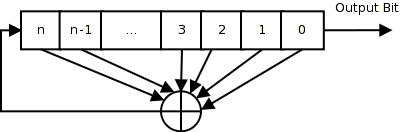
\includegraphics[scale=0.5]{images/lfsr}
    \caption{Linear feedback shift register (Fibonacci configuration)}
    \label{fig:lfsr-fib}
\end{figure}
Another type of LFSR is called a Galois configuration. It has the same
properties, but the feedback scheme is different: each bit in the tap sequence
is XORed with the output bit and replaced; the output bit then becomes the new
left-most bit (figure \ref{fig:lfsr-galois}).
\begin{figure}[htbp]
    \centering
    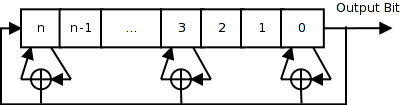
\includegraphics[scale=0.5]{images/lfsr_galois}
    \caption{Linear feedback shift register (Galois configuration)}
    \label{fig:lfsr-galois}
\end{figure}
A sequence generated by LFSR is linear by itself and therefore useless for
cryptography. It is possible to recover the LFSR structure from intercepting
only $2n$ bits of the generator using Berlekamp-Massey algorithm~\cite{joux:algorithmic_cryptanalysis}.

Feedback with carry shift registers (FCSR) are similar to LFSRs but instead of
XORing the tapping sequence bits are added to the carry register. The result
reduced modulo 2 becomes the feedback bit of the register and the result divided
by 2 becomes the new value of the carry register.

The carry register has to be at least $\log_2 t$, where $t$ is the number of
taps. Thus, before the carry register is
filled there are some states of FCSR that never repeat. The maximum period of
FCSR differs from the one of LFSR. It equals to $q - 1$, where $q$ is the
connection integer and defined as
\mbox{$q = 2 q_1 + 2^2 q_2 + 2^4 q_4 + \cdots + 2^n q_n - 1$}; $q$ has to be a prime
for which 2 is a primitive root. In fact not every initial state guarantees
maximum period of the register. That means the all pseudo-random sequence
generators based on FCSR will have a set of weak
keys~\cite{schneier:applied_cryptography:2}.

Non-linear feedback shift registers (NLFSR) use non-linear feedback function.
Such stream ciphers as Grain and Trivium are based on NLFSRs. The idea both
behind NLFSRs and FCSRs is to ensure high non-linearity of the output sequence.
However such non-linear behavior makes the analysis of such registers almost
impossible. The described registers are unpredictable --- they don't guarantee
maximal-period sequence, which also depends on the initial state of the register,
output sequences may have biases of zeroes and ones or contain long bit series.
Hereby, the advantage of these registers may at the same time lead to critical
flaw. Consequently, NLFSRs and FCSRs should be used with utmost caution.


\subsubsection{Clock control}

Clock control is one of several ways to introduce high nonlinearity in
pseudo-random sequence generated by linear feedback shift registers. The rate of
register clocking varies either depending on several LFSRs or on certain bits
of the register state~\cite{usm:streamciphers}. As will be shown further, the combination of clock
control, combination and filter generators allow to form a pseudo-random
sequence satisfying all statistic requirements and yet resistant to known
attacks.

\subsubsection{Generators}

The use of feedback shift registers for cryptographic applications is possible by
combining several registers into a single generator.

The technique of combining outputs of several
registers by a Boolean function is called \textit{combination generator}
(figure~\ref{fig:comb-gen}). The output sequence $s_t$ of a combination generator
composed on $n$ LFSRs is given by
\begin{equation}
    \label{eqn:comb-gen-seq}
    s_t = f(u_1, u_2, \cdots, u_n), \enspace \forall t \leq 0 \enspace,
\end{equation}

where $u_i$ denotes the sequence generated by the $i$-th LFSR and $f$ is a
function of $n$ variables~\cite{encyclopedia_of_cryptography}.
\begin{figure}[htbp]
    \centering
    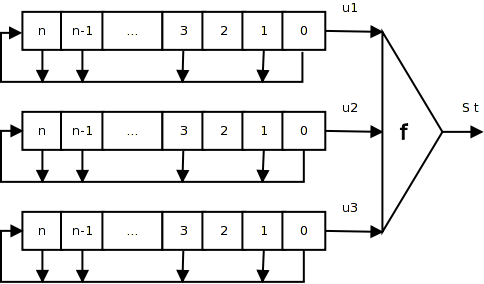
\includegraphics[scale=0.5]{images/comb-gen}
    \caption{Combination generator}
    \label{fig:comb-gen}
\end{figure}
The output of the $f$ function must be uniformly distributed and balanced in
order to produce pseudo-random sequences.

Linear complexity of the keystream generated by a combination generator composed
of $n$ LFSRs with primitive feedback polynomials combined by a Boolean function
$f$ equals to
\begin{equation}
    \label{eqn:lin-complexity}
    f(L_1, L_2, \cdots, L_n) \enspace,
\end{equation}

where the algebraic normal form of $f$ is evaluated over
integers and all lengths $L_1, \cdots, L_n$ are distinct and greater than 2.
High linear complexity of the generator is required to ensure that
Berlekamp-Massey algorithm is computationally infeasible.

Combination generators are vulnerable to correlation attacks based on
recovering the initial states of all LFSRs from the knowledge of some sequence
produced by the generator (known plaintext attack). In order to protect
generators from this kind of attacks, the LFSR feedback polynomials should not
be sparse to ensure a high correlation-immunity order of the combining function.
However the correlation-immunity of a balanced Boolean function of $n$ variables
is limited with $n - 1 - deg(f)$~\cite{encyclopedia_of_cryptography}. Tradeoffs
between high algebraic degree, high nonlinearity and high correlation-immunity
may be outwitted replacing the combining function by a finite state automaton
with memory.

\textit{Filter generators}, in distinction of combination generators, consist of
single LFSR and its state is filtered by a nonlinear
function~(figure~\ref{fig:filter-gen}). The output of the function is a
pseudo-random sequence formed by the generator. Just like in combination
generators the filtering function must be uniformly distributed and balanced.
\begin{figure}[htbp]
    \centering
    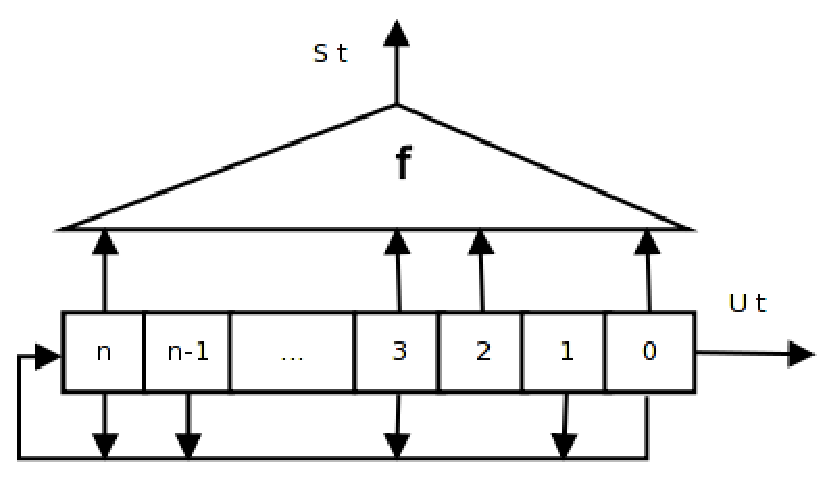
\includegraphics[scale=0.5]{images/filter-gen}
    \caption{Filter generator}
    \label{fig:filter-gen}
\end{figure}

Any filter generator can be represented by a corresponding combination generator
consisting of $n$ copies of the LFSR with shifted initial states when the
combining function complies the filtering function.

Filter generators are vulnerable to fast correlation and generalized inversion
attacks~\cite{canteaut:invattack}. Filtering function should be highly nonlinear
in order to resist the fast correlation attack. The inversion attack depends on
the largest spacing between two taps of the LFSR which conflicts with the
statement that LFSRs should use dense polynomials. Also the greatest common
divisor of all spaces between taps should be equal to 1 or else the inversion
attack could be simplified~\cite{encyclopedia_of_cryptography}.

Algebraic attacks are also applicable to filter generators since a keystream
bit can be represented by a function of $L$ initial bits of the LFSR. Therefore,
knowing $N$ keystream bits allows to form an algebraic system of $N$ equations
of $L$ variables. Usage of Gr\"obner bases (which may be viewed as nonlinear
generalization of Gaussian elimination for linear systems) enables an attacker
to lower the degree of equations until the recovery of LFSR initial state is
possible by solving the algebraic system even with filtering function of high
degree.

Some designs of LFSR-based generators that promise to be secure are considered
further.

\textit{Alternating stop-and-go generator} uses three LFSRs of different length.
LFSR-1 controls clocking of the other two. If output of LFSR-1 is 0, LFSR-3 is
clocked, if its output is 1, LFSR-2 is clocked. The output of the generator is
the XOR of LFSR-2 and LFSR-3.  A correlation attack on LFSR-1 exists, but it
does not threaten the generator's
security~\cite{schneier:applied_cryptography:2}.

\textit{Bilateral stop-and-go generator} uses two LFSRs of length $n$ and its
output bit equals to XOR of the outputs of each LFSR. The functioning of
the generator is described by algorithm~\ref{alg:stop-go-gen}.
\begin{algorithm}
    \caption{Bilateral stop-and-go generator functioning}
    \label{alg:stop-go-gen}

    \SetKw{Land}{and}
    \SetKwData{LfsrI}{LFSR-1}
    \SetKwData{LfsrII}{LFSR-2}
    \SetKwFunction{Output}{Output of}
    \SetKwFunction{Block}{Block}
    \DontPrintSemicolon

    \If{\Output{\LfsrII at time $t-1$} == $0$ \Land \;
    \Indp \Output{\LfsrII at time $t-2$} == $1$ \;}{
    \Block(\LfsrII at time $t$)
    }\;
    \If{\Output{\LfsrI at time $t-1$} == $0$ \Land \;
    \Indp \Output{\LfsrI at time $t-2$} == $1$ \Land \;
    \LfsrI clocked at time $t$ \;}{
    \Block(\LfsrII at time $t$)
    }\;
\end{algorithm}
So far no critical attacks on this generator have been presented. Another
alternative is filter generator that consists in forming cryptographically
strong pseudo-random sequence as some nonlinear function of a state of the
single register~\cite{robshaw:rsa:streamciphers}.

The idea behind the \textit{shrinking generator} is simple and uses two LFSRs.
Both of them are clocked each time: if the output of LFSR-1 is 1, then the
generator outputs bit from LFSR-2, otherwise both bits are discarded and the
LFSRs are clocked again. The generator is said to be secure if no sparse
polynomials are used in LFSRs, but the downside is irregular output rate.
This problem can be solved by buffering though it complicates implementation.

\textit{Self-shrinking generator} is similar to shrinking generator but uses
pairs of bits from a single LFSR. After clocking the register twice output bits
are analysed: if the first bit is 1, the output is the second bit; if the first
bit is 0, bits are discarded and the register is clocked again. This generator
is slower but requires less memory. However its properties are hard to analyse.

\subsubsection{T-functions}

A new building block for symmetric ciphers called T-function was introduced by
Klimov and Shamir in 2003~\cite{klimov:tfunc}. T-function is a class of
invertible mappings that mix arithmetic and boolean operations and process
full machine words.

Consider a construction where each input variable has $n$ bits, and $m$ input
variables are placed in $m$ rows of \mbox{$m \times n$ bit} matrix. Than a
T-function is defined by mapping
\begin{equation}
    \label{eqn:t-func}
    f: \mathbb{B}^{m \times n} \rightarrow \mathbb{B}^{k \times n} \enspace,
\end{equation}%

where $\mathbb{B} = \{0, 1\}$ and each $k$-th column of the output depends only on
the first $k$ columns of the input. In general, in order to compute the $k$-th
output bit only input bits $0, 1, \cdots, k$ must be known. Most machine
instructions are T-functions: negation, addition, subtraction, multiplication, left
shift, which is identical to multiplication by $2$. Any combination of
T-functions is also a T-function.

The name of such transformation refers to the triangular dependence of the following
form~\cite{dblp:conf/fse/klimovs05}:
\begin{equation}
    \left(
    \begin{array}{c}
        \left[ f(x) \right]_0 \\
        \left[ f(x) \right]_1 \\
        \left[ f(x) \right]_2 \\
        \vdots \\
        \left[ f(x) \right]_{n-1} \\
    \end{array} \right)%
    = \left(
    \begin{array}{c}
        f_0([x]_0) \\
        f_1([x]_0, [x]_1) \\
        f_2([x]_0, [x]_1, [x]_2) \\
        \vdots \\
        f_{n-1}([x]_0, \cdots, [x]_{n-2}, [x]_{n-1})
    \end{array} \right) \enspace,
\end{equation}

where $\left[ f(x) \right]_k$ is the $k$-th output column and
$[x]k-1, \cdots, [x]_0$ --- first $k$ input columns.

The primary advantage of T-functions is computation efficiency both in hardware
and software implementation on modern processors. Despite of having desirable
cryptographic properties, some functions revealed weaknesses to correlation,
algebraic and distinguishing attacks~\cite{mycrypt/kunzli_jm05} with a complexity of
$2^{32}$. Even though usage of T-functions is highly attractive, reasonable
security of such transformations should be proved first.


\section{Formulation of the problem}

In spite of advances in mathematic methods of modern cryptography, real world
security system often end up using vulnerable ciphers due to insufficient
preliminary analysis. By the time the security cryptoalgorithm is properly
studied, the cipher itself is already deployed in global system -- switching is
expensive and hard technologically.

In order to prevent such situations methods for efficient cryptographic security
analysis of ciphers need to be propagated and best practices for cryptographic
primitives design and evaluation provided. Most widely used cryptanalytic
methods (linear and differential cryptanalysis, etc.) are based on statistical
approach and require tremendous amount of data for sane evaluation. Even with
exponential growth of computational power it most probably will be impossible
neither in the near future nor any given time in future to apply these
statistical methods to modern full-scale ciphers.

To make statistical cryptanalytic methods somewhat applicable to ciphers used in
modern security systems the concept of baby-ciphers has been introduced. The
concept implied proportional shrinking of all transformations of the cipher in
order to get a baby-version -- still similar to the original cipher but its full
statistical analysis is computationally feasible. However the correspondence of
such statistical evaluation to the full-scale original cipher hasn't yet been
proved.

Nonetheless algebraic analysis of cryptoalgorithms and recent advances in
computational algebra allow to obtain systems of multivariate equations that
mathematically describe the behaviour of full-scale ciphers and require only few
pairs of \mbox{plaintext/ciphertext} for valid analysis. Most equations systems
for modern ciphers are still hard to compute, but the complexity gap for solving
full-scale system of equations is times smaller than for statistical methods to
analyze full-scale cipher.

Though the algebraic analysis method is promising, it is not yet widely used and
has been applied to only few ciphers. In order to perform algebraic analysis of
any cryptoalgorithm it first must be defined by a system of multivariate
non-linear equations. Therefore to make the algebraic cryptanalysis technique
commonly used by cryptologists some patterns and best practices in constructing
polynomial equations for modern ciphers must be made available to the public.
Not only the theoretical part is important for valid evaluation. The ready to
use reference software implementation with examples is the key wide
applicability of algebraic analysis methods.

In order to solve the described issues and enable aglebraic analysis efficiently
applicable for modern symmetric cipher following solutions need to be provided:

\begin{enumerate}
    \item develop guide lines for constructing system of non-linear equations for
modern ciphers as well as for individual transformations commonly used in modern
ciphers;
    \item describe the most efficient methods and provide best practices for
        solving algebraic equations systems;
    \item use provided methods for applying algebraic attack to actual ciphers;
    \item describe needed software tools and provide reference implementation
        for all steps of algebraic attack for easy reproduce and application to
        other ciphers.
\end{enumerate}



